% !TeX program = xelatex
% !TeX encoding = UTF-8
% Compile with XeLaTeX twice, or use the built-in LaTeX preview.
\documentclass[a4paper,11pt]{article}
\usepackage[T1]{fontenc}
\usepackage{lmodern}
\usepackage[margin=2.3cm,top=2.1cm,bottom=2.2cm]{geometry}
\usepackage{amsmath,amssymb}
\usepackage{booktabs,longtable,array}
\usepackage{graphicx}
\usepackage{placeins}
\usepackage{enumitem}
\usepackage{titlesec}
\usepackage{xurl}
\usepackage[unicode,hidelinks]{hyperref}
\hypersetup{pdftitle={STAT5291 NFL Project Proposal},pdfsubject={Bayesian hierarchical regression of receiver separation}}
\titleformat{\section}{\large\bfseries}{\thesection}{.6em}{}
\titleformat{\subsection}{\normalsize\bfseries}{\thesubsection}{.6em}{}
\titlespacing*{\section}{0pt}{1.2ex plus .3ex}{.7ex}
\titlespacing*{\subsection}{0pt}{1ex plus .2ex}{.4ex}
\setcounter{tocdepth}{1}
\linespread{1.12}
\setlength{\parskip}{.25em}
\setlength{\emergencystretch}{2em}
\setlength{\tabcolsep}{5pt}
\setlength{\LTpre}{.6em}
\setlength{\LTpost}{.6em}
\renewcommand{\arraystretch}{1.16}
\setlist[enumerate]{leftmargin=2.2em,itemsep=.2em,topsep=.3em}
\newcommand{\code}[1]{{\small\ttfamily #1}}
\newlength{\tablecontentwidth}
\setlength{\tablecontentwidth}{\dimexpr\textwidth-4\tabcolsep\relax}
\newcolumntype{P}[1]{>{\raggedright\arraybackslash}p{#1}}
\newcolumntype{R}[1]{>{\raggedleft\arraybackslash}p{#1}}
\begin{document}
\begin{center}
{\large STAT5291 Final Project Proposal\par}
\vspace{.6em}
{\LARGE\bfseries A Bayesian Hierarchical Analysis\par}
\vspace{.2em}
{\LARGE\bfseries of Combine Post-Turn Speed Change\par}
\vspace{.2em}
{\LARGE\bfseries and Rookie NFL Receiver Separation\par}
\end{center}
\vspace{.3em}

This project uses NFL Big Data Bowl 2027 data to examine whether a wide receiver's signed speed change after a candidate turn in a standardized Combine route drill is associated with rookie-season receiver separation, beyond the information provided by the conventional 40-yard dash time. The analysis centers on interpretable Bayesian hierarchical regression, distinguishing within-player differences across defensive coverages from between-player differences in coverage exposure. It addresses repeated observations, partial pooling, and parameter uncertainty. Throughout this proposal, ``post-turn speed change'' is shorthand for this provisional measurement; it is not treated as a validated measure of stable reacceleration ability.

Initial data checks, exploratory data analysis (EDA), and a window sensitivity analysis with fixed candidate turn times have been completed. The provisional sample contains 68 wide receivers, 11,405 player-play records, and 559 games. The final sample remains subject to a review of all candidate trajectories. No regression model has yet been fitted. The proposal therefore distinguishes verified descriptive findings from planned analyses and does not presume an association's direction or statistical significance.

\section{Research Questions and Scope}

\subsection{Background}

The 40-yard dash measures straight-line sprint performance, whereas receiving routes also require deceleration, changes of direction, and speed recovery. NFL Big Data Bowl 2027 provides both Combine trajectories and corresponding game data, allowing this project to examine the relationship between a specific pre-NFL test measurement and professional game performance.\cite{nfl}

Each player contributes multiple route observations across games, and observation counts vary substantially across players. Observations from the same game may also share tactical, opponent, and field conditions. The project therefore uses crossed player and game random effects rather than treating all player-play records as independent. The hierarchical model links player-level Combine measurements to play-level outcomes and partially pools estimates for players with limited observations.\cite{gelman}

\subsection{Primary Question}

Among wide receivers with eligible rookie-season passing-route records, how is signed speed change after a candidate Combine turn associated with separation at pass release, after adjusting for 40-yard dash time, draft cohort, route, pre-snap cushion, and game context, while distinguishing within-player and between-player coverage differences?

The primary parameter is $\beta_A$, the population regression coefficient for the standardized speed-change measurement. The analysis will report its posterior distribution, 95\% credible interval, and predicted distance differences on a practically interpretable scale. The near-zero unadjusted correlation observed in the EDA does not determine this conditional coefficient. A statistically clear positive association is not a prerequisite for a successful project.

\subsection{Secondary Questions}

\begin{enumerate}
\item Does adding the trajectory measurement improve predictions of separation for players excluded from model fitting, conditional on their game contexts?
\item How much player-level and game-level heterogeneity remains after adjustment? How does partial pooling affect estimates for players with few observations?
\item Does the conditional MAN--ZONE contrast within a player differ from the association corresponding to between-player differences in the proportion of MAN coverage faced?
\item In staged extensions, does the MAN--ZONE contrast vary across players, and can the trajectory measurement explain some of that heterogeneity?
\end{enumerate}

The project estimates conditional associations and gains in conditional prediction. Because it uses observed routes and coverage contexts, it is not a forecast based solely on information available before the draft. The sample does not identify the causal effect of reacceleration training, and the findings cannot automatically be generalized to all prospects, including those who never appear in an NFL game.

\section{Data Sources and Analytical Sample}

The data come from NFL Big Data Bowl 2027 and cover the 2023--2025 draft cohorts and their associated games. The primary analysis uses the following five tables and does not require processing all frame-level game-tracking files.

{\small
\begin{longtable}{@{}P{0.29\tablecontentwidth}P{0.37\tablecontentwidth}P{0.34\tablecontentwidth}@{}}
\caption{Data files and join keys}\label{tab:1}\\
\toprule
\textbf{File} & \textbf{Purpose} & \textbf{Join keys} \\
\midrule
\endfirsthead
\toprule
\textbf{File} & \textbf{Purpose} & \textbf{Join keys} \\
\midrule
\endhead
\bottomrule
\endlastfoot
\code{players.csv} & Player position and draft cohort & \code{nfl\_\allowbreak{}id} \\[.15em]
\code{combine\_\allowbreak{}results.csv} & 40-yard dash time and body measurements & \code{nfl\_\allowbreak{}id}, \code{draft\_\allowbreak{}year} \\[.15em]
\code{combine\_\allowbreak{}tracking.csv} & Speed change after a candidate turn & \code{nfl\_\allowbreak{}id}, \code{draft\_\allowbreak{}year}, \code{event\_\allowbreak{}id} \\[.15em]
\code{player\_\allowbreak{}play.csv} & Separation and play context & \code{nfl\_\allowbreak{}id}, \code{game\_\allowbreak{}id}, \code{play\_\allowbreak{}id} \\[.15em]
\code{games.csv} & Season and regular-season, preseason, or postseason classification & \code{game\_\allowbreak{}id} \\[.15em]
\end{longtable}
}

The downloaded files contain 510 players, including 106 with official position WR; \code{player\_\allowbreak{}play.csv} contains 314,197 records. Initial checks found no duplicate player keys, game keys, or player--game--play composite keys. Joining the player and game tables produced no unmatched records or row inflation. These counts refer to the actual downloaded files used in this project.

The observational unit is one wide receiver's route on one play in one game. Inclusion requires official position WR; game season equal to draft year; \code{season\_\allowbreak{}type = REG}; membership on the offensive team; a play not nullified by penalty; a pass result of complete, incomplete, or intercepted (\code{C}, \code{I}, \code{IN}); and observed route and separation measurements. Sacks and quarterback scrambles do not share the same pass-release outcome definition, so their missing separation values are not replaced with zero.

{\small
\begin{longtable}{@{}P{0.6\tablecontentwidth}R{0.19\tablecontentwidth}R{0.21\tablecontentwidth}@{}}
\caption{Sample selection}\label{tab:2}\\
\toprule
\textbf{Stage} & \textbf{Unique WRs} & \textbf{Player-play records} \\
\midrule
\endfirsthead
\toprule
\textbf{Stage} & \textbf{Unique WRs} & \textbf{Player-play records} \\
\midrule
\endhead
\bottomrule
\endlastfoot
Eligible rookie regular-season routes with separation at pass release & 79 & 14,733 \\[.15em]
Observed 40-yard dash time and complete primary controls & 72 & 12,450 \\[.15em]
Also matched to right-curl drill trajectories & 69 & 11,664 \\[.15em]
Passing the provisional turn and complete-window checks & 68 & 11,405 \\[.15em]
\end{longtable}
}

The final row defines the provisional sample, with 23, 26, and 19 players in the three respective cohorts. The final selection flow will be updated after trajectory review, with reasons reported for excluded players and records. Model comparisons will use the same final intersection sample.

\section{Variables and Measurement Construction}

\subsection{Outcome}

Let $S_{ipg}$ denote \code{separation\_\allowbreak{}at\_\allowbreak{}pass\_\allowbreak{}forward} for player $i$ on play $p$ in game $g$: the distance in yards to the nearest defender at pass release. This measures available space at one instant, not catch probability, maximum separation over the entire route, or overall player value.

Among the 14,733 eligible records, 3,006 correspond to targeted receivers and 11,727 to non-targeted receivers; separation is observed in both groups. The primary analysis retains both groups rather than conditioning inclusion on being targeted. All eligible distances are positive. In this broader sample, the median is 2.62 yards and the mean is 3.11 yards. These are descriptive statistics, not fitted-model results.

The primary outcome is $y_{ipg}=\log(S_{ipg})$, where $S$ is expressed numerically in yards. This corresponds to a lognormal conditional distribution on the original scale and ensures positive predicted distances. Posterior predictive checks will assess whether this distribution adequately captures the tails and any heteroscedasticity.

\subsection{Primary Predictor}

The primary predictor is derived from \code{CURL\_\allowbreak{}ROUTE\_\allowbreak{}RIGHT} and defined as the signed average rate of speed change over the 0.5 seconds following a geometric candidate turn. Only \code{entity\_\allowbreak{}type = PLAYER} records are retained, excluding ball trajectories that carry the same player identifier. Tests are separated by player and \code{event\_\allowbreak{}id}, and frames are sorted by time. This definition describes the quantity directly calculated without assuming that the selected instant marks the start of acceleration.

The provisional turn detector compares displacement directions over the 0.5 seconds before and after each candidate instant. Both displacement speeds must be at least 2 yards per second, the angle must be at least 45 degrees, and both windows must be complete. The eligible instant with the largest angle is selected as $t_{\mathrm{cut}}$. This is a feasibility-screening rule. Before fitting, trajectory plots will be reviewed to check whether the selected point represents the intended route break rather than a post-catch or end-of-drill movement.

For eligible test $r$ of player $i$, define

\begin{equation}
A_{ir}=\frac{s_{ir}(t_{\mathrm{cut}}+0.5)-s_{ir}(t_{\mathrm{cut}})}{0.5}.
\end{equation}

Here, $s$ is scalar speed and $A_{ir}$ is measured in yards per second squared. If a player has multiple eligible tests, their median defines $A_i$. Negative values are retained: they indicate that speed is lower at the end of the window than at its start, not necessarily that every frame within the window shows deceleration. The observed negative example indicates that the geometric turn time need not coincide with the onset of acceleration. All candidate tests will be reviewed using the trajectories themselves before fitting, with rules and exclusions documented. Windows, negative values, and players will not be selected according to their association with game outcomes.

Only one of the 68 provisional players has two eligible tests. For almost every player, $A_i$ is therefore effectively a single measurement, not a validated estimate of stable ability. The primary analysis relates observed test performance to game outcomes. Window and smoothing sensitivity analyses will address measurement uncertainty without attempting to identify test--retest reliability from the very limited repeat data.

\subsection{Other Variables}

{\small
\begin{longtable}{@{}P{0.3\tablecontentwidth}P{0.29\tablecontentwidth}P{0.41\tablecontentwidth}@{}}
\caption{Predictors and grouping variables}\label{tab:3}\\
\toprule
\textbf{Variable} & \textbf{Level and coding} & \textbf{Role} \\
\midrule
\endfirsthead
\toprule
\textbf{Variable} & \textbf{Level and coding} & \textbf{Role} \\
\midrule
\endhead
\bottomrule
\endlastfoot
\code{forty} & Player level; seconds; standardized & Assess information beyond straight-line sprint performance; a lower time is faster \\[.15em]
\code{draft\_\allowbreak{}year} & Player level; cohort fixed effects & Adjust for cohort and concurrent environment; no duplicate season effects under the rookie-season restriction \\[.15em]
\code{route\_\allowbreak{}ran} & Play level; categorical & Adjust for route-specific spatial demands \\[.15em]
\code{team\_\allowbreak{}coverage\_\allowbreak{}man\_\allowbreak{}zone} & $M_{ipg}$: MAN = 1, ZONE = 0 & Construct within-player deviations and mean exposure; unknown values are not coded as ZONE \\[.15em]
$M^W_{ipg}=M_{ipg}-\bar M_i$ & Play level; centered within player & Describe the conditional MAN--ZONE contrast within a player \\[.15em]
$\bar M_i$ & Player level; MAN proportion (0--1) & Describe between-player differences in coverage composition \\[.15em]
\code{cushion} & Play level; yards; centered and standardized & Adjust for pre-snap distance to the primary defender \\[.15em]
\code{down} & Play level; categorical & Adjust for the offensive down \\[.15em]
\code{yards\_\allowbreak{}to\_\allowbreak{}go} & Play level; continuous; standardized & Adjust for the yards needed on the play \\[.15em]
Player and game identifiers & Grouping variables & Define crossed random intercepts \\[.15em]
\end{longtable}
}

The defender used to measure \code{cushion} may differ from the nearest defender at pass release. Consequently, their distance difference is not directly interpreted as space created by the receiver. Height, weight, and alignment may be added in prespecified sensitivity analyses; numerous highly correlated body measurements will not be included simultaneously in the primary model.

\section{Exploratory Data Analysis: Preliminary Findings}

The figures and tables in this section were produced by rejoining, filtering, and processing the five downloaded source tables, using the turn-detection rule defined in Section 3. The drill, window, and exclusion thresholds were not adjusted in response to NFL outcomes. The sample-selection and missingness analyses begin with 79 WRs with eligible pass-release observations. The remaining figures use the current candidate sample: 68 players, 11,405 player-play records, and 559 games. Unless otherwise stated, player-level figures contain one observation per player, whereas play-level distribution plots include all eligible records. All findings below are descriptive; no hierarchical regression has yet been fitted.

\subsection{Sample Composition, Missingness, and Selection}

Figure~\ref{fig:eda-sample} shows the sample reductions associated with complete-case filtering and trajectory matching. The candidate sample contains 23, 26, and 19 players from the 2023, 2024, and 2025 cohorts, respectively. In the broader sample of 79 players, 40-yard times are missing for 7 players; short-shuttle and three-cone times are missing for 50 and 56 players, respectively. The latter two measures are therefore unsuitable as required controls in the main model. The cohort-specific missingness rate for cushion is approximately 4.65\%--5.27\%, while the missingness rate for MAN/ZONE labels is below 0.1\% in every cohort.

\begin{figure}[htbp]
\centering
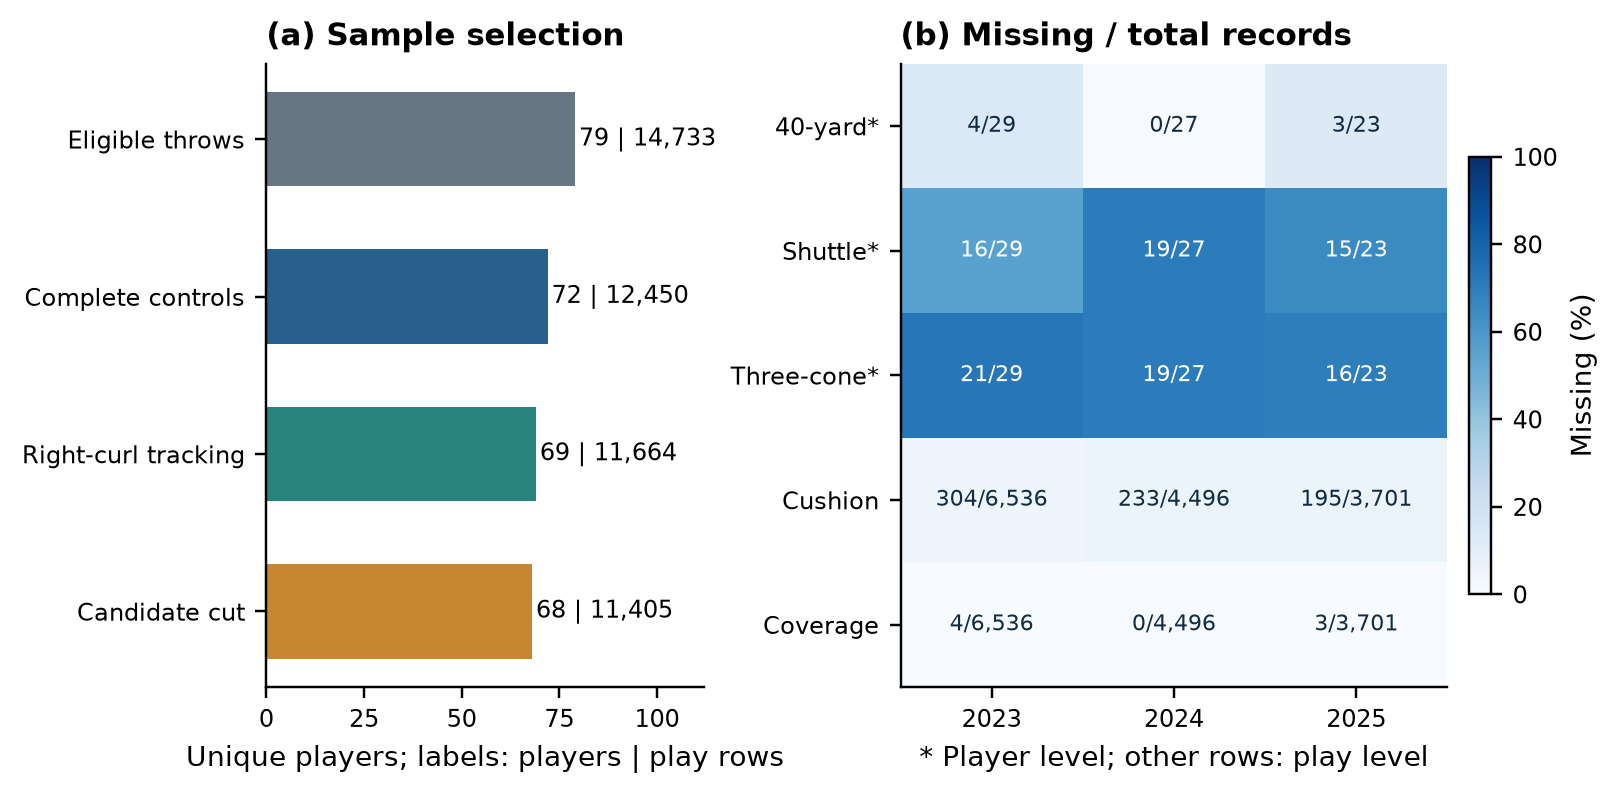
\includegraphics[width=\linewidth]{images/eda_01_sample_missingness.png}
\caption{Sample selection and missingness by cohort. In the left panel, bar lengths represent the number of unique players; adjacent labels report player counts followed by player-play counts. The right panel displays missing counts divided by totals, with color indicating the percentage missing. For test results marked with an asterisk, the denominator is the number of players in that cohort; for cushion and coverage, it is the number of eligible player-play records in that cohort.}
\label{fig:eda-sample}
\end{figure}
\FloatBarrier

Table~\ref{tab:eda-selection} compares the 68 included players with the 11 excluded players within the same 79-player baseline sample. Excluded players have greater mean height and weight, and their distribution of participation counts also differs. These differences suggest that complete-case filtering and trajectory matching may yield a selected sample. Only 4 excluded players have observed 40-yard times, so the observed mean for this small subset cannot establish that sprint performance is similar between the groups. In addition, the 68 included players originally contributed 12,012 eligible pass-release records, of which 607 were omitted from the candidate sample because play-level controls were incomplete. Player-level comparisons do not replace an assessment of this record-level missingness.

\begin{table}[htbp]
\centering\small
\caption{Descriptive comparison of included and excluded players (baseline: 79 eligible WRs)}
\label{tab:eda-selection}
\begin{tabular}{@{}P{0.40\tablecontentwidth}P{0.30\tablecontentwidth}P{0.30\tablecontentwidth}@{}}
\toprule
Measure & Included in candidate sample & Not included in candidate sample \\
\midrule
Unique players & 68 & 11 \\
Players in 2023 / 2024 / 2025 & 23 / 26 / 19 & 6 / 1 / 4 \\
40-yard time, seconds: mean (SD) & 4.457 (0.084), $n=68$ & 4.438 (0.097), $n=4$ \\
Height, inches: mean (SD) & 72.27 (2.13) & 73.50 (2.98) \\
Weight, pounds: mean (SD) & 194.19 (14.63) & 200.55 (16.74) \\
Baseline plays per player: median [quartiles] & 176.5 [59.0, 270.5] & 192.0 [123.0, 404.5] \\
\bottomrule
\end{tabular}
\par\smallskip
\begin{minipage}{\linewidth}\footnotesize
Note: Each player is counted once. Height and weight are observed for 68 and 11 players in the two groups, respectively; 40-yard summaries use nonmissing values only. Play counts here precede complete-case filtering of controls and therefore differ from the final candidate play counts in Figure~\ref{fig:eda-clusters}. No significance tests were conducted between the groups.
\end{minipage}
\end{table}
\FloatBarrier

\subsection{Trajectory and Measurement Quality Checks}

Figure~\ref{fig:eda-trajectory} presents two right-side curl trials: the trial with $A$ closest to the median among eligible events and the trial with the smallest $A$. Examples were selected solely from Combine trajectories, without using NFL outcomes. Both have complete 0.5-second windows before and after the candidate point and a sampling interval of 0.1 seconds.

In the first example, the candidate point is near the visible change in direction, and the subsequent 0.5-second increase in speed yields $A=2.80$. In the second, although the trial passes the 45-degree turn threshold, speed falls from 2.94 yd/s at the candidate point to 1.79 yd/s after 0.5 seconds, yielding $A=-2.30$; speed continues to decline after the candidate point. This demonstrates that the time of maximum geometric heading change need not mark the start of acceleration. The current metric should therefore be interpreted as signed speed change after a candidate point. This negative value is retained in all subsequent figures; negative values must not be deleted, or cut points shifted, to manufacture positive results.

\begin{figure}[htbp]
\centering
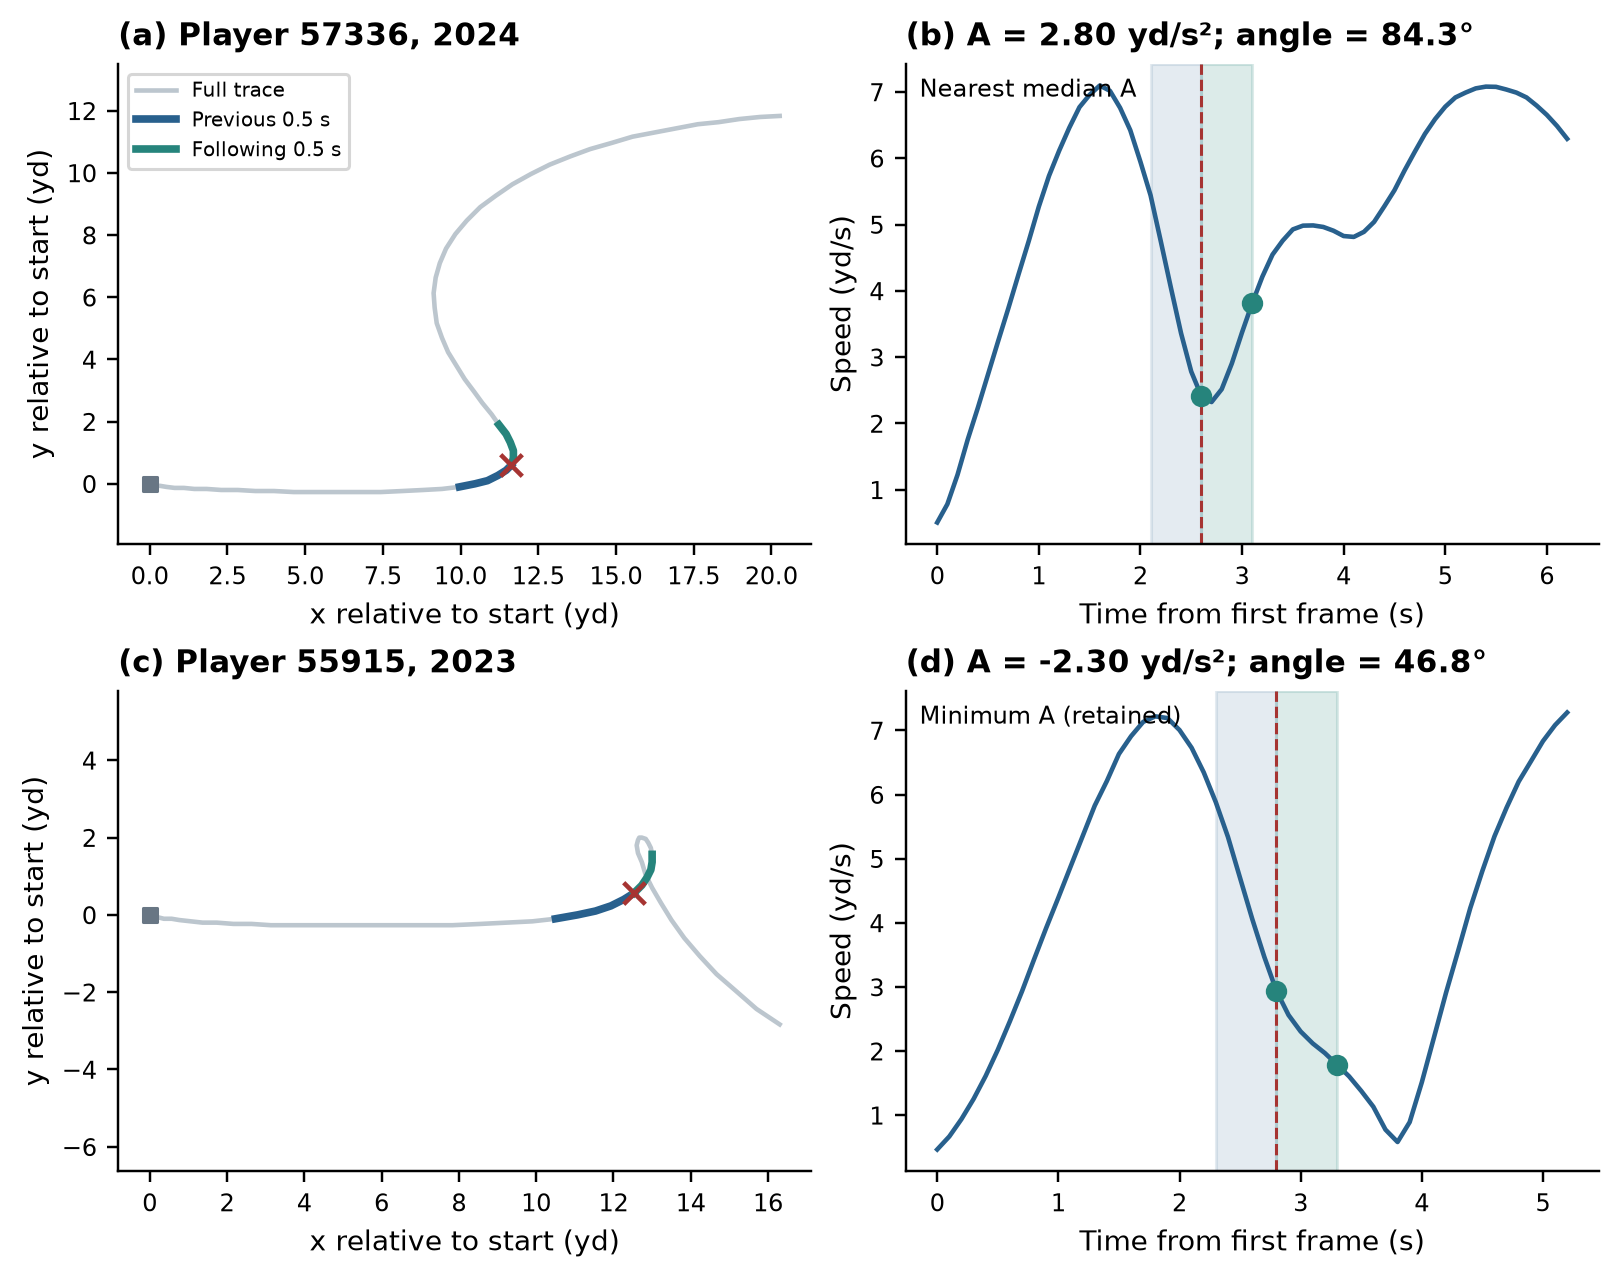
\includegraphics[width=\linewidth]{images/eda_02_trajectory.png}
\caption{Two-dimensional trajectories and speed-time curves for two trials. The left panels use equal axis scales and translate the starting location to the origin. Squares mark the start, and red crosses mark the candidate turn point; blue and green segments denote the preceding and following 0.5 seconds, respectively. The right panels shade the same windows, with a red dashed line at the candidate point. The upper and lower examples are player 57336 (2024) and player 55915 (2023), respectively. They illustrate checks of the measurement rule and do not establish that all trajectories have been validated.}
\label{fig:eda-trajectory}
\end{figure}
\FloatBarrier

\subsection{Separation Distributions and Game Context}

In the candidate sample, separation has a mean of 3.07 yards, a median of 2.61 yards, an interquartile interval of [1.39, 4.25] yards, and a range of 0.28--17.68 yards. Sample skewness on the original scale is 1.28, reflecting a relatively long right tail. After log transformation, skewness is $-0.20$, and the marginal distribution is more symmetric (Figure~\ref{fig:eda-outcome}). This supports using a log transformation as the starting point for the main model, but does not establish that residuals conditional on the covariates are normal or homoskedastic; those assumptions must still be checked after fitting.

Median separation under MAN and ZONE is 1.53 and 3.08 yards, respectively, based on 3,208 and 8,197 records. Distributions also differ substantially across route types. Direct comparisons of players' raw mean separation may therefore reflect differences in their coverage and route composition. These unadjusted group differences are not causal effects of coverage or route type.

\begin{figure}[htbp]
\centering
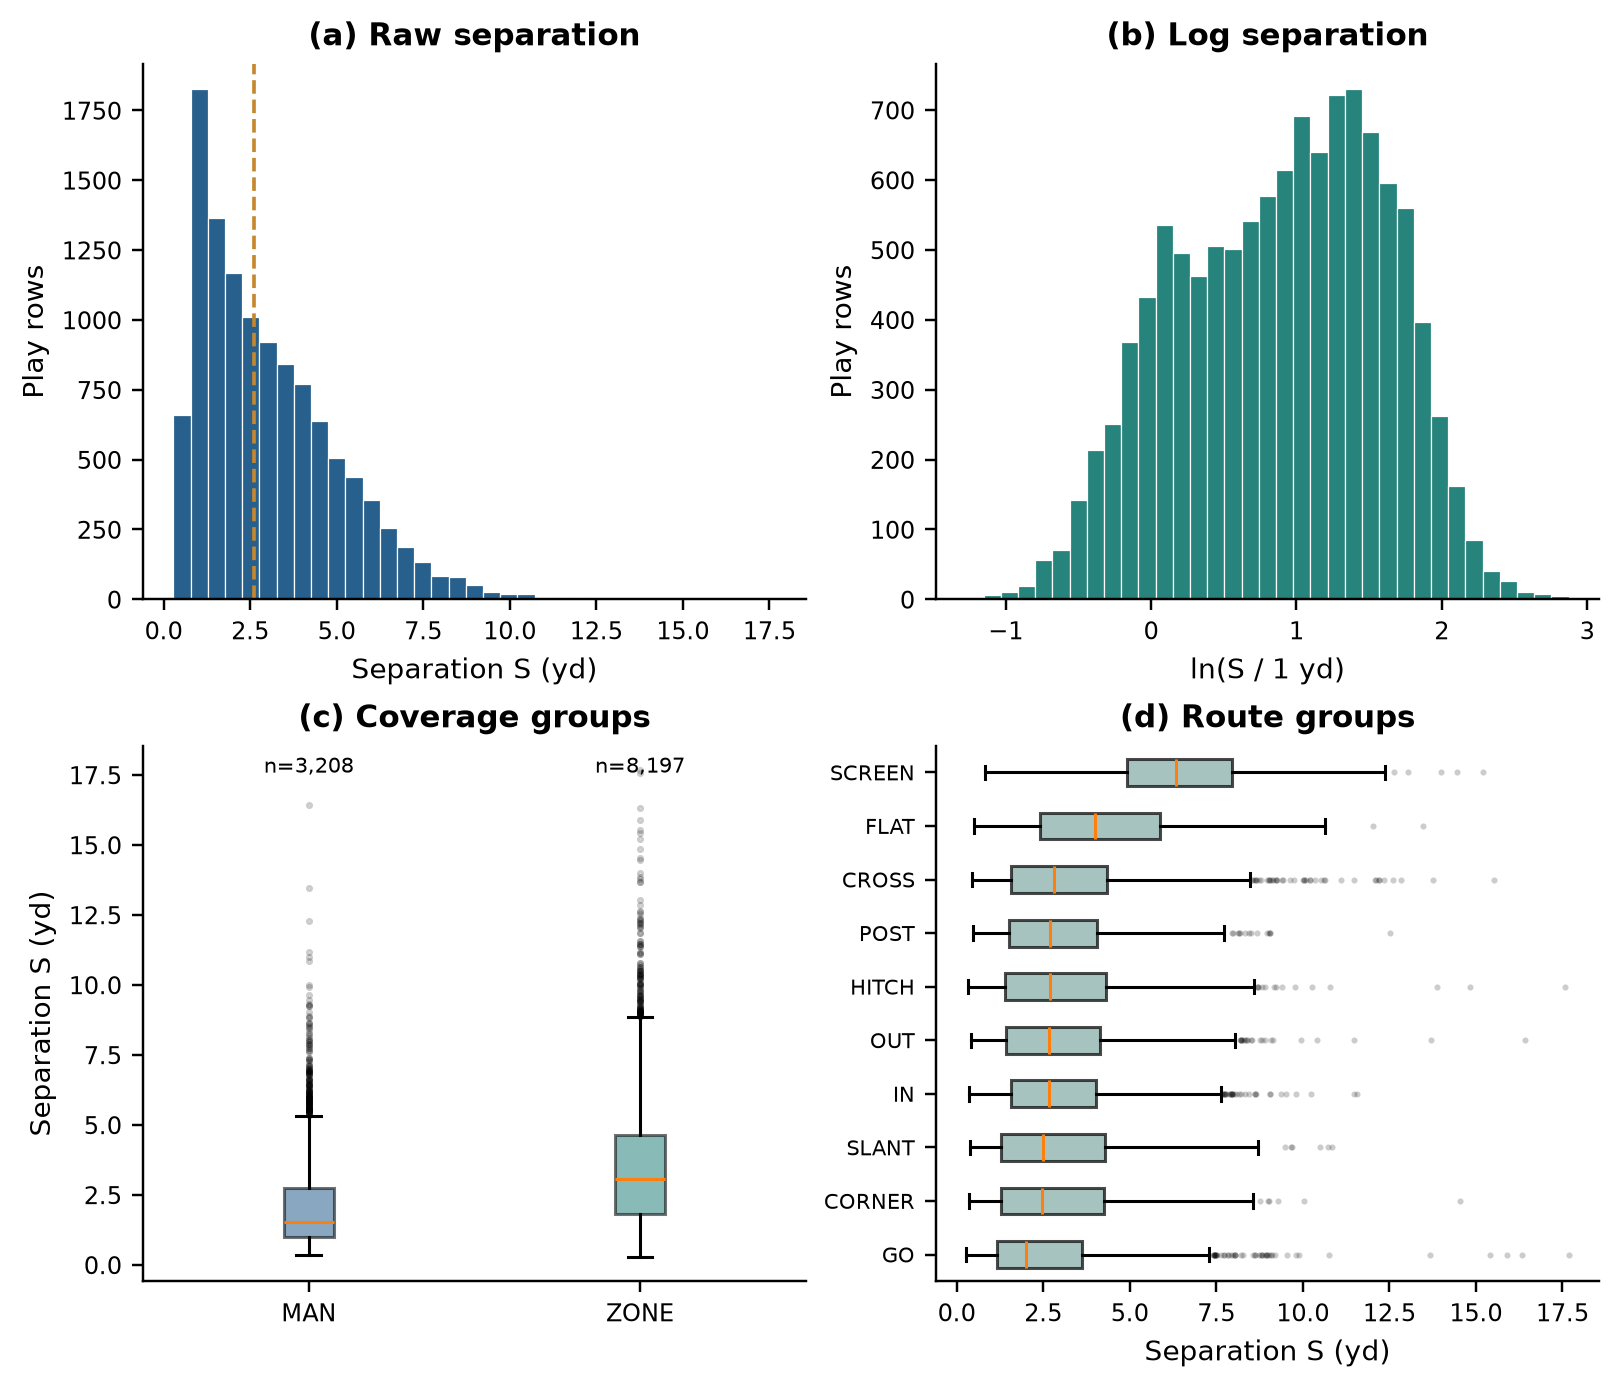
\includegraphics[width=\linewidth]{images/eda_03_outcome.png}
\caption{Outcome distributions in the candidate sample, including all 11,405 player-play records. (a) Histogram on the original scale, with a dashed line marking the median; (b) histogram on the natural-log scale; (c) MAN/ZONE boxplots; (d) route boxplots ordered by median. Boxes show the interquartile interval, internal lines mark medians, and whiskers extend to the most extreme observations within 1.5 times the interquartile range. Points retain observations beyond the whiskers. The right tail is not truncated, and player-play records are not assumed to be independent.}
\label{fig:eda-outcome}
\end{figure}
\FloatBarrier

\subsection{Player-Level Metrics and 40-Yard Times}

Figure~\ref{fig:eda-player} retains one $A_i$ per player; for the only player with two eligible trials, it uses their median. Across 68 players, $A_i$ has a median of 2.80, an interquartile interval of [2.08, 3.26], and a range of $-2.30$--5.03 yd/s$^2$. The mean 40-yard time is 4.457 seconds, with a standard deviation of 0.084 seconds.

Giving each player equal weight, the Pearson correlation between $A_i$ and 40-yard time is $-0.082$, and the Spearman correlation is $-0.121$. Linear and monotonic associations are both weak in the current sample, with no indication of strong bivariate collinearity. This does not establish statistical independence or guarantee predictive gains from the trajectory metric. The figure also identifies draft cohorts; cohort differences will remain controlled as planned.

\begin{figure}[htbp]
\centering
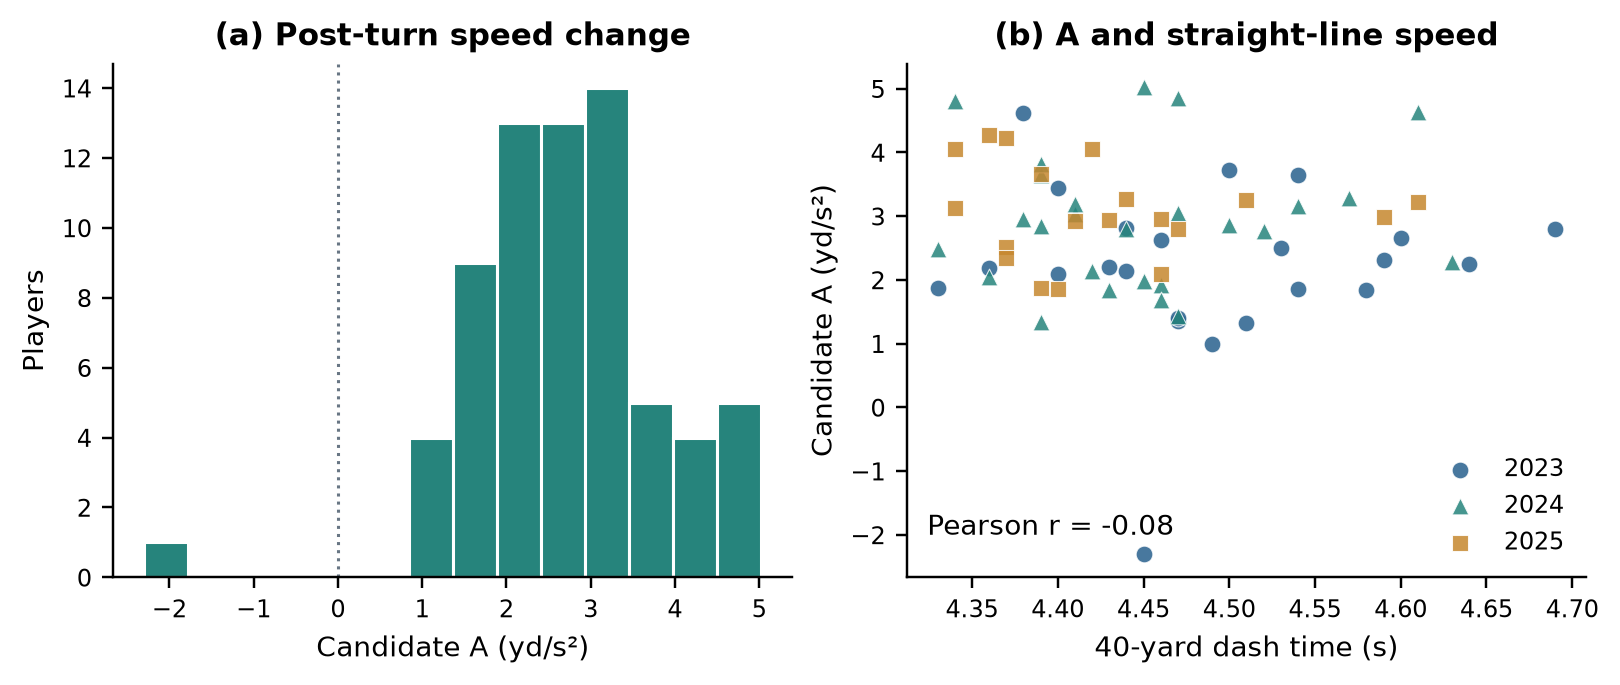
\includegraphics[width=\linewidth]{images/eda_04_player_metrics.png}
\caption{Player-level metric distributions and relationships ($n=68$). (a) Distribution of the candidate speed-change metric, with a dashed line at zero; (b) relationship with 40-yard time. Color and shape jointly identify draft cohorts; shorter 40-yard times indicate faster sprints. All eligible players are retained, including the only player with a negative $A_i$.}
\label{fig:eda-player}
\end{figure}
\FloatBarrier

\subsection{Repeated Observations and Coverage Structure}

The median number of candidate plays per player is 165.5, with an interquartile interval of [51.5, 259.25] and a range of 1--431. The median number of games is 14, with a range of 1--17 (Figure~\ref{fig:eda-clusters}). Observation counts are highly unbalanced, and some players contribute very little data, so the precision of player means varies considerably. Partial pooling in a hierarchical model can reflect these differences, while player-level predictors still have only 68 independent player-level sources of variation.

Of the 68 players, 64 have observations under both MAN and ZONE, and 46 have at least 20 records under each. This provides some information for examining within-player MAN--ZONE differences, but is insufficient to estimate every player's random slope precisely. In addition, 698 of the 10,707 distinct game plays contain two sample WRs, accounting for 1,396 observations. This supports examining residual dependence within shared plays in a sensitivity analysis.

\begin{figure}[htbp]
\centering
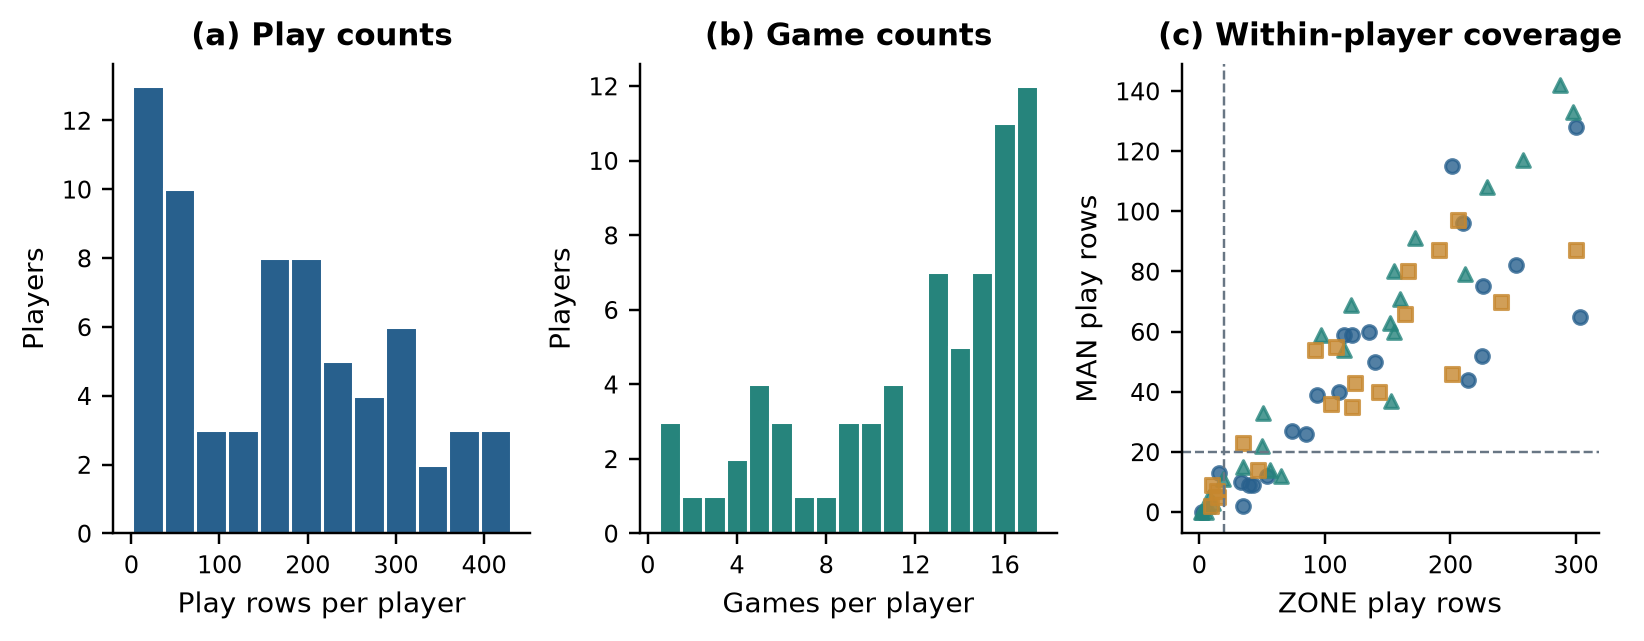
\includegraphics[width=\linewidth]{images/eda_05_repeated_observations.png}
\caption{Repeated-observation structure for the 68 candidate players. (a) Plays per player; (b) games per player; (c) MAN and ZONE record counts for the same player, with dashed lines at 20 records per category. Colors and shapes follow the cohort coding in Figure~\ref{fig:eda-player}. The threshold of 20 describes data coverage and is not an additional sample-exclusion rule.}
\label{fig:eda-clusters}
\end{figure}
\FloatBarrier

\subsection{Unadjusted Player-Level Association}

Figure~\ref{fig:eda-association} pairs each player's $A_i$ with their mean log separation. Point area increases with play count, while color and shape identify the draft cohort. With equal weight assigned to each player, the Pearson correlation is $-0.024$ and the Spearman correlation is $0.013$, indicating no clear linear or monotonic relationship at this marginal, aggregated level. Means for players with few observations may be highly unstable, so their vertical positions in the figure should not be interpreted as ability rankings.

This finding does not predetermine a zero coefficient in the subsequent hierarchical model, nor does it support a positive effect. The central task remains to estimate the conditional association and its uncertainty after controlling for 40-yard time, cohort, route, coverage, and cushion, and to assess predictive gains through an M0/M1 comparison on the same sample. The metric or player sample should not be changed merely because the current correlation is near zero.

\begin{figure}[htbp]
\centering
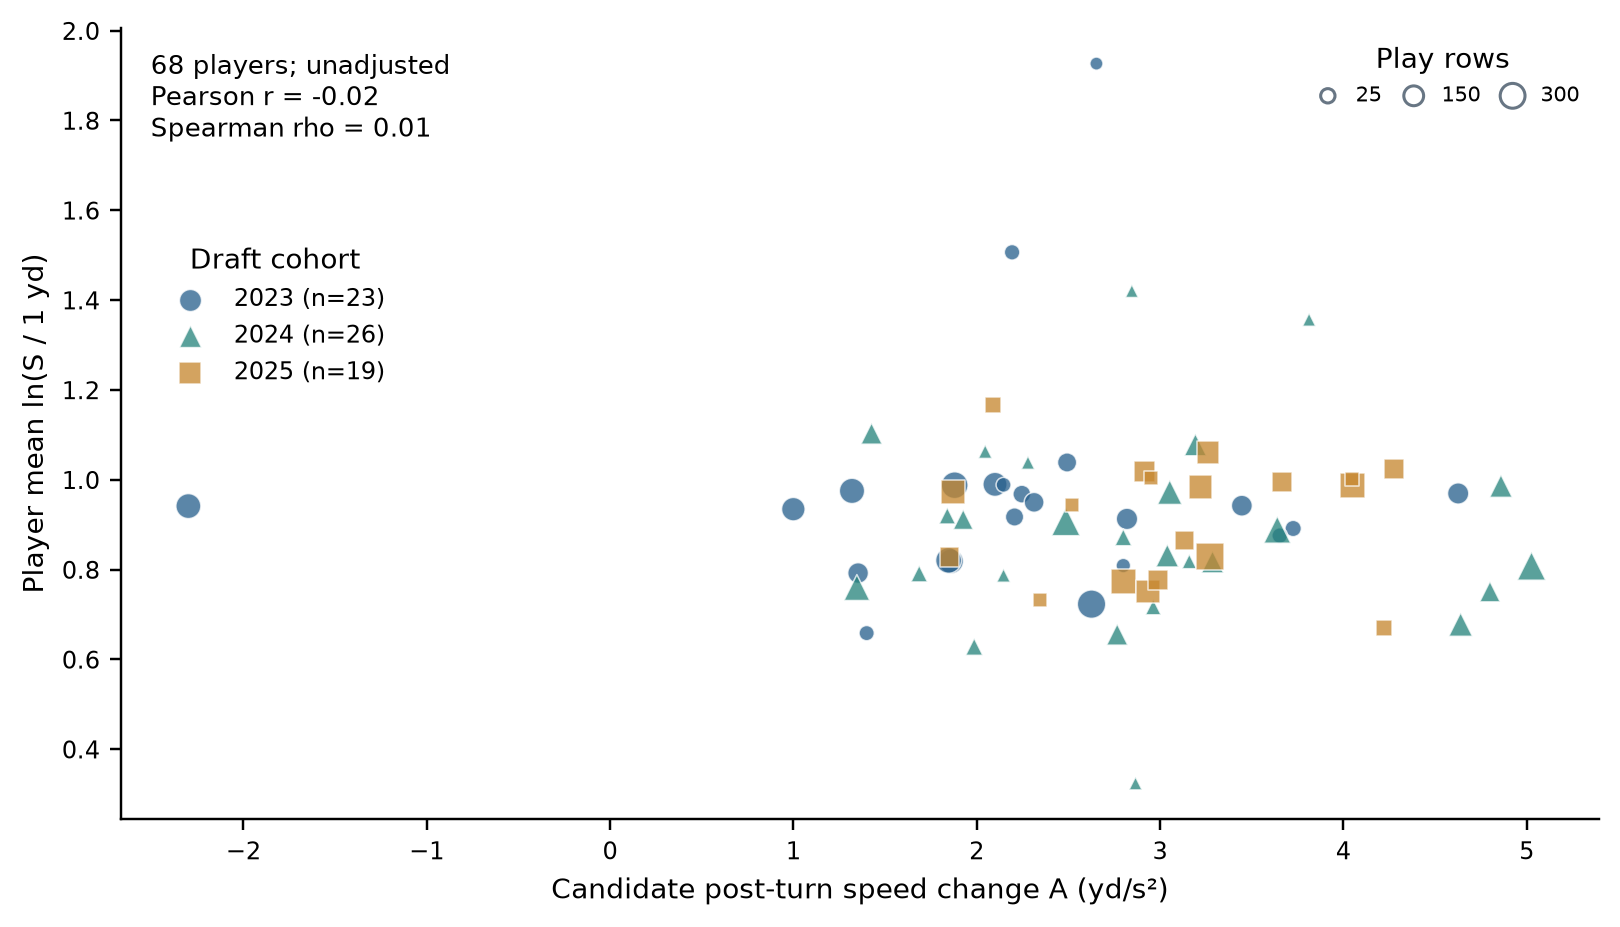
\includegraphics[width=\linewidth]{images/eda_06_initial_association.png}
\caption{Descriptive relationship between the candidate trajectory metric and players' mean log separation. Each point represents one player (68 in total), with point area increasing with play count; the legend illustrates the corresponding sizes. Correlations assign equal weight to players, are not weighted by play count, and do not adjust for game context. No significance test treats repeated player-play records as independent observations.}
\label{fig:eda-association}
\end{figure}
\FloatBarrier

This EDA describes the candidate sample and checks selected trajectories; it has not established measurement validity for all 69 eligible trials. Section 6 reports additional preliminary sensitivity results for 0.3-, 0.5-, and 0.7-second windows while keeping the original candidate turn points fixed. All trajectories still require review before formal fitting, together with an assessment of smoothing and turn-location rules. These steps will be based solely on measurement quality, without seeking stronger correlations with NFL outcomes. If a rule change alters the sample, coverage under each rule will be reported and results compared on the common sample.

\section{Hierarchical Models}

\subsection{Implications of the EDA for Model Design}

The marginal distribution of log separation is more symmetric than the distribution on the original scale, so a lognormal conditional distribution remains the starting point for the main model. The large differences in the number of observations per player support retaining crossed player and game random intercepts with partial pooling, without imposing an additional minimum number of appearances to exclude players with few observations. Differences across coverage types and routes support continued adjustment for game context. The main model also decomposes MAN into a within-player deviation and a player's average exposure to distinguish associations at the two levels. This is a modeling choice motivated by the research question; differences in group medians alone do not establish that the decomposition is necessary. Further changes to random slopes or the error distribution will be guided by diagnostics after fitting, rather than by marginal histograms alone.

\subsection{Main Model}

Let $\widetilde A_i$ and $\widetilde F_i$ denote the standardized candidate speed-change measure and 40-yard dash time, respectively, with each player counted once when calculating the standardization parameters. The vector $\mathbf W_{ipg}$ contains route, cushion, down, and yards to go. Let $\mathcal O_i$ be the set of plays included in the analysis for player $i$, with $n_i=|\mathcal O_i|$, and define:

\begin{equation}
\bar M_i=\frac{1}{n_i}\sum_{(p,g)\in\mathcal O_i}M_{ipg},
\qquad M^W_{ipg}=M_{ipg}-\bar M_i.
\end{equation}

The proportion $\bar M_i$ remains on its 0--1 scale and is not additionally standardized. The main model, M1, is:

\begin{equation}
\begin{aligned}
y_{ipg}&\sim N(\mu_{ipg},\sigma^2), \\
\mu_{ipg}&=\alpha_i+\lambda_W M^W_{ipg}+\boldsymbol\gamma^T\mathbf W_{ipg}+u_g.
\end{aligned}
\end{equation}

\begin{equation}
\begin{aligned}
m_i&=\alpha_0+\beta_A\widetilde A_i+\beta_F\widetilde F_i
       +\lambda_B\bar M_i+\delta_{c(i)}, \\
\alpha_i&\sim N(m_i,\tau_{\mathrm{player}}^2), \\
u_g&\sim N(0,\tau_{\mathrm{game}}^2).
\end{aligned}
\end{equation}

Here, $c(i)$ denotes draft year, with one year designated as the reference category. The intercept $\alpha_i$ represents a player's baseline level at that player's own average coverage exposure, with the other controls at their reference values. Its population mean is explained by Combine performance, the MAN proportion, and draft year. The game effect $u_g$ captures remaining differences shared within the same game. Players participate in multiple games, and a game may contain several sampled players, so the structure is crossed rather than simply nested.

The coefficient $\lambda_W$ describes the conditional difference in log separation between MAN and ZONE for the same player, holding the other controls fixed. The coefficient $\lambda_B$ describes the between-player conditional association of the MAN proportion with baseline performance, evaluated at each player's own average coverage exposure. The coefficient $\lambda_B$ corresponds to a proportion increase of 1, or 100 percentage points; an increase of 10 percentage points corresponds to $0.1\lambda_B$. The within-player and between-player coefficients are not constrained to be equal. Including group means of predictors in the group-level model distinguishes these two associations, but does not automatically eliminate correlations between other covariates and remaining player differences.\cite{bafumi}

The main parameter of interest is $\beta_A$. In M1, holding the other variables, including $\bar M_i$, fixed and using the same random-effects distribution, $\exp(\beta_A)$ is the conditional median separation ratio associated with a one-standard-deviation increase in the speed-change measure, where the standard deviation is calculated at the player level. Posterior predictions will also translate the results into differences measured in yards. The quantity $\exp(\mu)$ is not used directly as the arithmetic mean separation; mean predictions must account for residual uncertainty and uncertainty in the relevant random effects.

The model estimates $\beta_A$ from differences between players. It cannot identify a causal effect by comparing the within-player values of $A_i$, which do not vary. The hierarchical distribution assumes exchangeability of remaining player differences conditional on the covariates. Team tactics, quarterbacks, and unobserved player characteristics may still be associated with the predictors.

\subsection{Priors and Estimation}

Regularizing priors will be used. Initial choices are $\alpha_0\sim N(\log 3,1^2)$ for the intercept and $N(0,0.5^2)$ for standardized continuous predictors, categorical contrasts, and year coefficients. The priors $\lambda_W,\lambda_B\sim N(0,0.5^2)$ correspond, respectively, to a MAN--ZONE contrast and a change across the full 0--1 range of the MAN proportion. Player and game standard deviations receive $\operatorname{HalfNormal}(0,0.5^2)$ priors, and the residual standard deviation receives a $\operatorname{HalfNormal}(0,1^2)$ prior. Here, HalfNormal denotes the corresponding zero-mean normal distribution restricted to the positive half-line. The priors will not be made nearly degenerate merely because the current marginal correlation involving $A_i$ is close to zero.

Before fitting, prior predictive checks will assess whether these scales generate implausible distances too frequently. The sensitivity of the main conclusions to wider priors will also be examined. Bayesian estimation will use Stan or an R interface, with multiple chains and checks of $\widehat R$, effective sample sizes, and divergences. The targets are $\widehat R<1.01$ for the main parameters, no unresolved divergences, and Monte Carlo error small enough not to affect interval estimates or predictive comparisons.

\subsection{Staged Extensions}

Grouped posterior predictions from the main model will be examined first. The first planned extension, M2, adds a player-specific MAN slope to M1 while retaining the between-player term for $\bar M_i$:

\begin{equation}
\begin{aligned}
\lambda_i&=\lambda_W+v_i, \\
v_i&\sim N(0,\tau_{\lambda}^2).
\end{aligned}
\end{equation}

In the play-level model, $\lambda_iM^W_{ipg}$ replaces $\lambda_WM^W_{ipg}$, and $\tau_\lambda$ receives a $\operatorname{HalfNormal}(0,0.5^2)$ prior. The 64 players observed under both coverage types provide a basis for attempting this extension, but do not establish in advance that the slopes have substantial heterogeneity. For players observed under only one coverage type, $M^W_{ipg}=0$, so their records provide no direct information about their own within-player slopes; their slope predictions rely mainly on the population level.

If the sampling and predictive diagnostics for M2 are satisfactory, a cross-level interaction will be considered as a secondary extension, M3:

\begin{equation}
\lambda_i=\lambda_W+\kappa\widetilde A_i+v_i,
\qquad \kappa\sim N(0,0.5^2).
\end{equation}

The coefficient $\kappa$ describes the conditional association between the tracking measure and the within-player MAN--ZONE difference. In this model, holding $M^W_{ipg}$ and the other variables fixed, a one-standard-deviation increase in $A_i$ corresponds to a conditional median separation ratio of $\exp(\beta_A+\kappa M^W_{ipg})$; $\beta_A$ alone describes the association at $M^W_{ipg}=0$. The initial extension assumes that the player intercept residual $\alpha_i-m_i$ is independent of $v_i$. If this assumption needs to be relaxed, a bivariate normal distribution with an $\operatorname{LKJ}(2)$ prior on the correlation matrix will be used as an additional sensitivity analysis.

No player-specific random slope will be assigned to $A_i$, which is constant within a player. Remaining dependence among multiple WRs on the same play will also be assessed; if needed, a play random intercept nested within game will be added in a sensitivity model. Random slopes, cross-level interactions, correlation parameters, and additional levels will not all be introduced in the first model.

\section{Feasibility Evidence and Main Limitations}

\subsection{Data Coverage and Sources of Information for Hierarchical Estimation}

Figure~\ref{fig:feasibility-support} presents available information alongside measurement limitations. The candidate sample contains 23, 26, and 19 players across the three cohorts, permitting between-player comparisons while controlling for cohort fixed effects. Of the 68 players, 46 have at least 20 records under both MAN and ZONE; 18 have records under both but fewer than 20 in at least one category; and 4 have records under only one category. Most players therefore exhibit within-player variation in coverage, supporting a within-player coverage term in the main model and random slopes as a subsequent extension. The threshold of 20 describes coverage only and is not an additional exclusion rule.

However, 67 players have only one eligible Combine trial, and only 1 has two. These data support an analysis of the association between the observed trajectory metric and NFL outcomes, but cannot establish population test-retest reliability or justify treating each observation as an error-free measure of individual ability.

\begin{figure}[htbp]
\centering
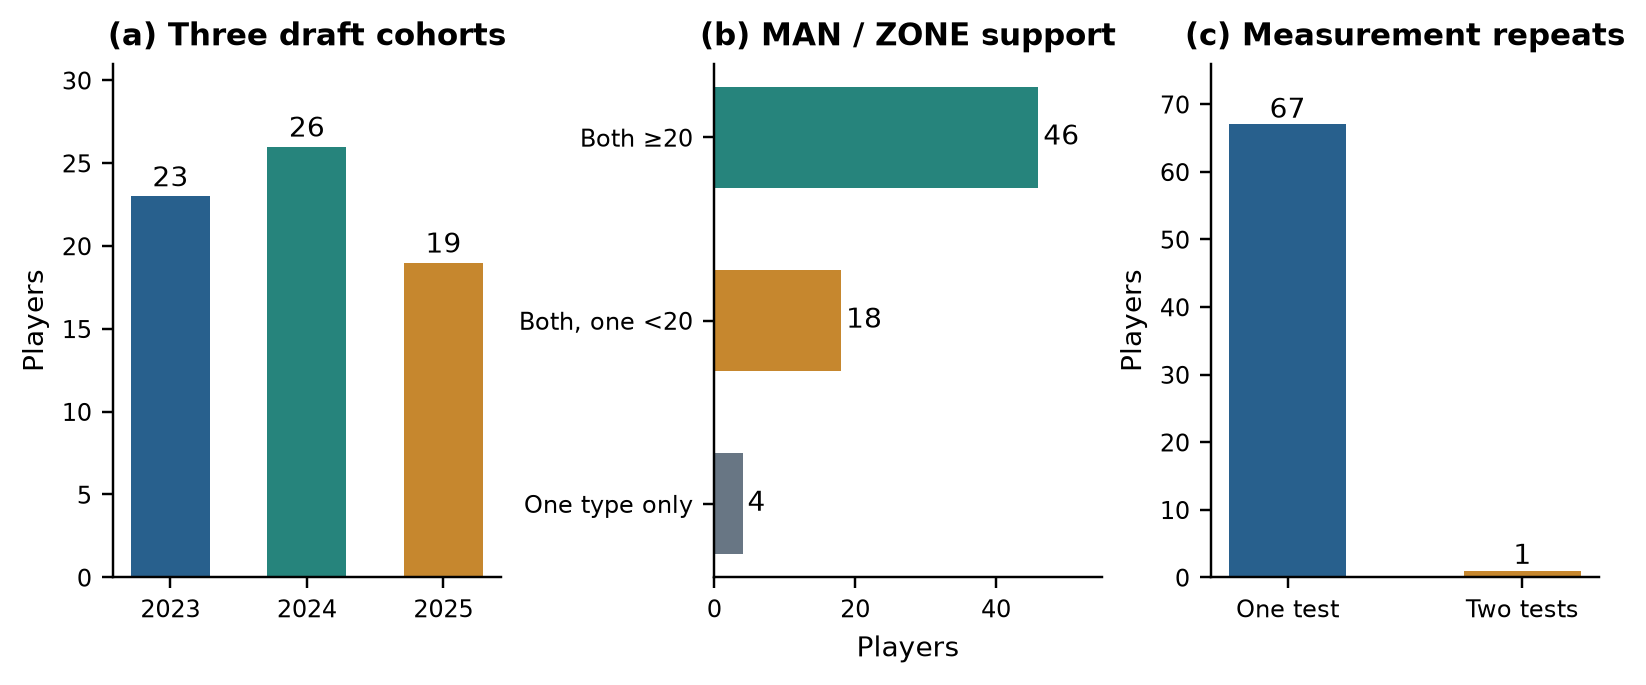
\includegraphics[width=\linewidth]{images/feasibility_01_data_support.png}
\caption{Data support and measurement limitations for the hierarchical analysis. (a) Candidate player counts across three draft cohorts; (b) three mutually exclusive MAN/ZONE exposure groups, totaling 68 players; (c) eligible Combine trials per player. The first two panels show the sources of player-level information and within-player coverage variation, while the third shows the scarcity of repeated measurements. Sample counts alone do not establish adequate statistical power or a nonzero true effect.}
\label{fig:feasibility-support}
\end{figure}
\FloatBarrier

The main analysis requires only five tables and does not require processing all frame-level game trajectories. Data preparation and figure generation have already been completed, and the computational scale is suitable for a course project. Regression fitting and diagnostics remain to be implemented. The 11,405 player-play records do not constitute the same number of independent player-level observations: $\beta_A$ primarily relies on comparisons among 68 players. The main model therefore retains a small set of player-level predictors and uses regularizing priors. The feasibility claim is that the model can be implemented and evaluated, not that weak effects are guaranteed to be detectable.

\subsection{Window Sensitivity with Fixed Turn Points}

To examine how speed differences depend on window length, the candidate turn points determined by the original 0.5-second geometric rule, the event set, and the quality filters were held fixed while calculating:

\begin{equation}
A_{ir}(w)=\frac{s_{ir}(t_{\mathrm{cut}}+w)-s_{ir}(t_{\mathrm{cut}})}{w},
\qquad w\in\{0.3,0.5,0.7\}\ \mathrm{s}.
\end{equation}

Every window retains the original 69 events and 68 players. Values were aggregated using each player's median across events and compared on the common sample. Relative to the 0.5-second window, the 0.3-second window has a Pearson correlation of 0.929 and a Spearman correlation of 0.873; the corresponding correlations for the 0.7-second window are 0.967 and 0.945 (Figure~\ref{fig:feasibility-window}). The same single player has a negative metric under all three windows, with no sign changes. Thus, with candidate points fixed, players' relative rankings are fairly stable across this prespecified set of windows.

Absolute values nevertheless differ: relative to the 0.5-second metric, the median absolute differences for the 0.3- and 0.7-second metrics are 0.49 and 0.27 yd/s$^2$, respectively, and the maximum absolute differences are 1.22 and 0.95. High correlations do not make the numerical values interchangeable, validate the candidate turn locations, or replace independent repeat trials. The main analysis retains the original 0.5-second definition, with subsequent regressions assessing conclusions under alternative windows. The primary result will not be selected according to which window produces a stronger association.

\begin{figure}[htbp]
\centering
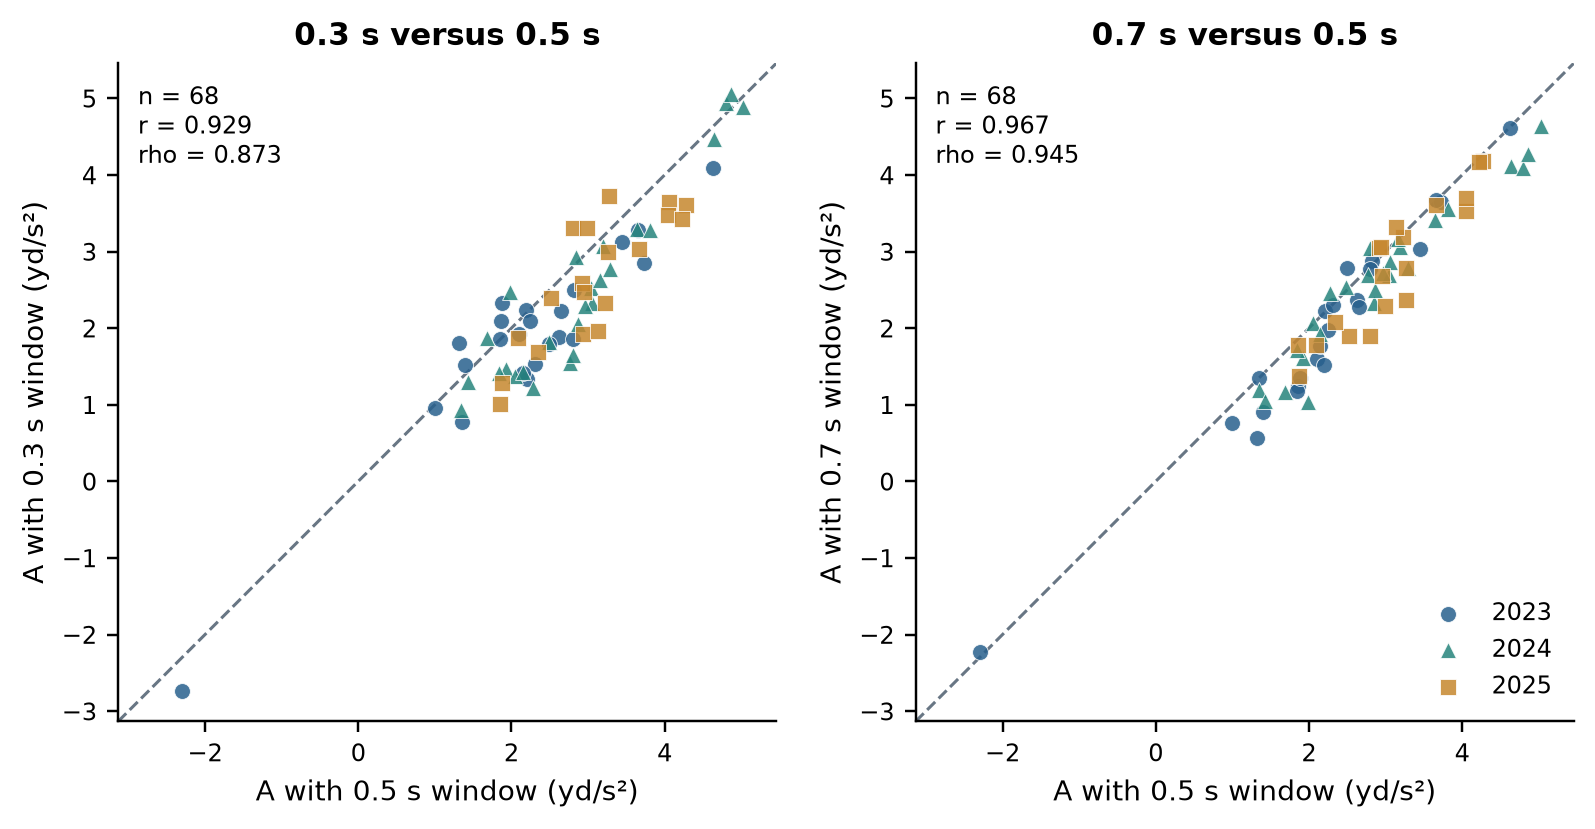
\includegraphics[width=\linewidth]{images/feasibility_02_window_sensitivity.png}
\caption{Window sensitivity with candidate turn points held fixed. Each point represents one player (common sample $n=68$). The horizontal axis shows the original 0.5-second metric; the vertical axes show the 0.3- and 0.7-second metrics, respectively. Dashed lines indicate equality. Colors and shapes identify draft cohorts; $r$ and $\rho$ denote Pearson and Spearman correlations. This check changes only the forward speed-difference window. It does not search for new turn points, alter smoothing rules, or use NFL outcomes for selection.}
\label{fig:feasibility-window}
\end{figure}
\FloatBarrier

\subsection{Remaining Selection and Dependence Issues}

Regarding measurement, speed differences may still depend on turn location, smoothing, and the minimum displacement-speed filter. All candidate trajectories must be reviewed before formal fitting, and any exclusions documented. The window check above does not replace this step, and records will not be excluded based on the sign of $A_i$ or the direction of a model coefficient.

Regarding missingness, 72 of the 79 players in the broader sample have observed 40-yard times. Among eligible pass-release records, cushion is missing for 732 records and MAN/ZONE for 7. Section 4 compares included and excluded players and identifies the 607 records lost within the included-player group. The main model begins with complete cases, followed by sensitivity analyses of missing-data handling. Its results cannot be interpreted as unbiased estimates for all rookies, and simple mean imputation will not replace a discussion of the missingness mechanism. Short-shuttle and three-cone times remain unsuitable as required predictors because of limited coverage.

Regarding clustering, 698 of the candidate sample's 10,707 distinct plays contain two sample WRs, so dependence within shared plays should be examined. Team and player membership also overlap substantially: in the earlier complete-case sample of 72 players, 47 of the 60 team-season combinations contain only one sample WR. An additional team-season intercept may therefore be difficult to distinguish from the player intercept and is omitted from the main model for now. The within-/between-player decomposition of MAN clarifies the interpretation of coverage associations, but does not automatically give $\beta_A$ a causal interpretation.

\section{Model Evaluation and Next Steps}

\subsection{Model Evaluation}

Two core models will be compared. M0 includes the conventional 40-yard dash time, draft year, game context, within-player and between-player MAN terms, and player and game random intercepts. M1 adds $\widetilde A_i$ to M0, as specified in Section 5. Both models use the same final players and plays, with identical remaining priors and data-processing rules. M2 adds a random MAN slope to M1. Only when supported by sampling and predictive diagnostics will the interaction $\widetilde A_i\times M^W_{ipg}$ be considered as the secondary extension M3. Whether the interaction is judged significant will not determine whether the main research question is retained.

Five-fold cross-validation will group observations by player, balancing the number of players from each draft year across folds as far as possible. All plays for a player will be assigned to the same fold. Standardization parameters will be estimated only from the training data; for $A_i$ and 40-yard dash time, the mean and standard deviation will count each training player once. For a held-out player, unknown random effects will be predicted from the population level without using that player's game outcomes to estimate an intercept or slope. Effects for games represented in training will be estimated using training data only; effects for unseen games will be predicted from the population distribution. The primary evaluation concerns generalization to new players conditional on observed game contexts, rather than prediction of an unknown future season from pre-draft information alone.\cite{loo}

For a training player, $\bar M_i$ will be calculated from that player's training plays. For a held-out player, $\bar M_i$ will be calculated only from the given MAN/ZONE labels for the set of plays to be predicted, without using separation or any other outcome variable. Because the evaluation conditions on the full set of game contexts, this proportion is an input to conditional prediction, not a feature known before the draft. If the objective changes to sequential, online prediction of individual plays, the analysis must instead use historical exposure known at the time of prediction or model unknown exposure; future coverage labels cannot be used in advance. All models will receive exactly the same predictive information within each fold.

Evaluation metrics will include MAE and RMSE on the original yard scale, posterior predictive interval coverage, and predictive log density. When comparing different conditional distributions, predictive log densities will be calculated on the same original separation scale. The primary summaries will first be calculated within each player and then averaged with equal weight for each player; results weighted by the number of plays will also be reported. Uncertainty in model differences will likewise be summarized at the player level so that a few players with many appearances do not dominate the evaluation.

Posterior predictive checks will compare the overall and group-specific separation distributions, upper tails, player means, and MAN/ZONE differences, and will examine predictive dispersion across coverage and route groups. A relatively symmetric marginal distribution of log separation does not establish conditional normality or homoscedasticity. If grouped predictions reveal systematic differences in dispersion, the first adjustment will allow the residual standard deviation to vary between MAN and ZONE. If the tails or distributional shape remain inadequately described, positive conditional distributions such as the Gamma will be compared, maintaining the same predictive evaluation scale.\cite{stanppc}

The main robustness analyses will cover the prespecified time windows and smoothing rules, a shared-play random intercept, prior scales, the handling of missing cushion values, and additional physical or alignment controls. The original single MAN term will serve as a comparison to assess how the within-player/between-player decomposition affects $\beta_A$. If needed, a player-mean term for cushion will also be added, rather than extending all controls simultaneously in the first model. A lack of predictive improvement does not establish that the true association is exactly zero.

\subsection{Implementation Sequence and Deliverables}

{\small
\begin{longtable}{@{}P{0.19\tablecontentwidth}P{0.48\tablecontentwidth}P{0.33\tablecontentwidth}@{}}
\caption{Implementation sequence and expected deliverables}\label{tab:5}\\
\toprule
\textbf{Stage} & \textbf{Tasks} & \textbf{Expected deliverables} \\
\midrule
\endfirsthead
\toprule
\textbf{Stage} & \textbf{Tasks} & \textbf{Expected deliverables} \\
\midrule
\endhead
\bottomrule
\endlastfoot
1 Measurement verification & Build on the completed window checks, review all candidate trajectories, and finalize quality rules & Measure definition, exclusion records, and final sample flow \\[.15em]
2 Analysis data update & Retain the completed preliminary EDA, update figures for the final sample, and construct $M^W_{ipg}$ and $\bar M_i$ & Analysis data, variable dictionary, and final EDA figures \\[.15em]
3 Main models & Run prior predictive checks, fit M0 and M1 with the coverage decomposition, and assess sampling and posterior predictions & Parameter posteriors, partial-pooling plots, and effects on the original scale \\[.15em]
4 Validation and extensions & Conduct grouped cross-validation and sensitivity analyses; assess M2 first and attempt M3 when supported by diagnostics & Model comparisons on the same sample and robustness results \\[.15em]
5 Reporting & Integrate the research questions, methods, results, and limitations & Final report, presentation materials, and reproducible analysis code \\[.15em]
\end{longtable}
}

If the main association is close to zero or its interval is wide, the report will describe the range of effects that can or cannot be ruled out at the current sample size and measurement precision. If the tracking measure is unstable under reasonable identification rules, the report will state the measurement limitations and restrict the main conclusions to observed performance in a single drill attempt, without claiming to have identified a stable measure of player ability.

\begin{thebibliography}{9}
\bibitem{nfl}
National Football League.
\emph{NFL Big Data Bowl 2027 Data Description}.
\href{https://www.kaggle.com/competitions/nfl-big-data-bowl-2027/data}{Official Kaggle data description}.
Player counts, missingness, and record counts in this proposal are based on direct inspection of the downloaded files on October 22, 2026.

\bibitem{gelman}
Gelman, A. (2006).
Multilevel (Hierarchical) Modeling: What It Can and Cannot Do.
\emph{Technometrics}, 48(3), 432--435.
\href{https://sites.stat.columbia.edu/gelman/research/published/multi2.pdf}{Author's publicly available version}.

\bibitem{bafumi}
Bafumi, J., and Gelman, A. (2006).
\emph{Fitting Multilevel Models When Predictors and Group Effects Correlate}.
Prepared for the Annual Meeting of the Midwest Political Science Association.
\href{https://statmodeling.stat.columbia.edu/wp-content/uploads/2006/04/Bafumi_Gelman_Midwest06.pdf}{Authors' publicly available conference paper}.

\bibitem{loo}
Vehtari, A. \emph{Cross-validation FAQ}.
\href{https://mc-stan.org/loo/articles/online-only/faq.html}{Official loo methodological guidance}.

\bibitem{stan}
Stan Development Team.
\emph{Stan User's Guide --- Regression Models}.
\href{https://mc-stan.org/docs/stan-users-guide/regression.html}{Guidance on hierarchical regression and priors}.
\bibitem{stanppc}
Stan Development Team.
\emph{Stan User's Guide --- Posterior and Prior Predictive Checks}.
\href{https://mc-stan.org/docs/stan-users-guide/posterior-predictive-checks.html}{Guidance on posterior predictive checks}.
\end{thebibliography}

\end{document}
